% =====================================================================
% EDICION EN ESPANOL de formalizing-transversal-matroids-in-lean4.tex.
% Traducir es revisar: toda correccion de fondo detectada aqui se vuelca
% tambien en el original ingles, no solo en la traduccion.
% Matroides transversales en Lean 4 -- la arquitectura de conjuntos tight
% y la obstruccion canonica.  First bead of the TotD strand drawn from the
% list "Theorems by Women Mathematicians".
% Authors: Carles Marín (Claude, Anthropic, as AI assistant).
% Style: clones the house line of godsil-gutman-lean.tex /
% neumann-separation-lean.tex: story-driven, one question per section,
% key formulas framed, Lean names in the tables, scope stated exactly.
% Build: pdflatex formalizing-transversal-matroids-in-lean4.tex (twice).
% Verified against the Lean source 2026-07-21:
%   lake build Theorems.TransversalObstruction  -> 1164 jobs, exit 0
%   #print axioms on the five headline theorems -> propext,
%   Classical.choice, Quot.sound only.  Toolchain leanprover/lean4:v4.32.0,
%   Mathlib revision 84fdd0bfb8e85237f54b9617cca79c6198d40a75 (2026-07-15),
%   local checkout E:\Mathlib\mathlib4.  Every priority/absence claim is
%   pinned to that revision and itemised in the Priority section.  The running example is
%   re-derived exhaustively by check_canonical_obstruction.sage before
%   every figure is drawn.
% =====================================================================
\documentclass[11pt]{article}
\usepackage[T1]{fontenc}
\usepackage[spanish,es-noshorthands]{babel}
\usepackage{lmodern}
\usepackage{amsmath,amssymb,amsthm,booktabs,graphicx,hyperref,tabularx,array}
\usepackage{xurl}
\usepackage[table]{xcolor}
\definecolor{tmteal}{HTML}{1B6F8C}
\definecolor{tmband}{HTML}{DCE7EB}
\definecolor{tmamber}{HTML}{E08A1E}
\definecolor{tmplum}{HTML}{7B4B94}
\definecolor{tmgrey}{HTML}{B9C2CC}
\usepackage[margin=1in]{geometry}
\usepackage{microtype}
\usepackage{float}
\usepackage[most]{tcolorbox}
\usepackage{tikz}
\usetikzlibrary{arrows.meta,positioning,calc,fit,decorations.pathreplacing}
\setlength{\emergencystretch}{2em}
% Keep figures inline: a float should not claim a page it does not fill.
\renewcommand{\topfraction}{0.86}
\renewcommand{\bottomfraction}{0.72}
\renewcommand{\textfraction}{0.10}
\renewcommand{\floatpagefraction}{0.80}
\setlength{\intextsep}{9pt plus 2pt minus 2pt}
\setlength{\textfloatsep}{11pt plus 2pt minus 3pt}
\newtheorem{theorem}{Teorema}
\newtheorem{lemma}{Lema}
\newtheorem{proposition}{Proposición}
\newtheorem{corollary}{Corolario}
\newcommand{\lean}[1]{\texttt{#1}}
\newcommand{\N}{\mathrm{N}}
\hypersetup{colorlinks=true,linkcolor=tmteal,citecolor=tmteal,urlcolor=tmteal}
\newtcbox{\keybox}{on line,boxrule=0.9pt,colframe=tmteal,colback=tmband!40,
  arc=3pt,left=8pt,right=8pt,top=5pt,bottom=5pt}
\newcommand{\keyeq}[1]{\begin{center}\keybox{$\displaystyle #1$}\end{center}}
\newtcolorbox{contribbox}[1]{colframe=tmamber,colback=tmamber!8,arc=3pt,boxrule=0.9pt,
  title=\textbf{#1},coltitle=white,colbacktitle=tmamber}
\newtcolorbox{recipebox}[1]{colframe=tmteal,colback=tmband!35,arc=3pt,boxrule=0.8pt,
  title=\textbf{#1},coltitle=white,colbacktitle=tmteal}

\title{\bf El conjunto que dice no\\[4pt]
  \large\normalfont Matroides transversales en Lean~4: una prueba del axioma de aumento
  por conjuntos \emph{tight}, y la obstrucción canónica que hace posible}
\author{Carles Mar\'in\thanks{Formalizado con asistencia de un sistema de IA (Claude,
Anthropic); las matemáticas son clásicas, y toda afirmación, delimitación de alcance y
limitación es responsabilidad del autor. Lo que \emph{no} está formalizado se expone sin
adornos en la Sección~\ref{sec:boundary}, y quien certifica las pruebas es el núcleo de
Lean, no el asistente.}\\[3pt]
  \normalsize Investigador independiente\\
  \normalsize \texttt{karlesmarin@gmail.com}}
\date{Julio de 2026}

\begin{document}
\maketitle

\begin{abstract}
Mathlib tiene el teorema de los matrimonios de Hall. Mathlib tiene matroides. En la revisión
contra la que se ha verificado este trabajo (\lean{84fdd0bf}, 15-07-2026) nada une ambas cosas:
todo matroide de \lean{Matroid/Constructions.lean} es trivial (\lean{emptyOn}, \lean{loopyOn},
\lean{freeOn}, \lean{uniqueBaseOn}), y ninguno se construye a partir de datos combinatorios. Este
artículo cierra ese hueco para el puente clásico entre ambas, el \emph{teorema del matroide
transversal} de Edmonds--Fulkerson y, de forma independiente, de Mirsky--Perfect: para una familia
finita $A=(A_0,\dots,A_{t-1})$ de conjuntos finitos, los transversales parciales de $A$ son
exactamente los conjuntos independientes de un matroide. Presento una formalización completa y sin
\lean{sorry} en Lean~4 sobre Mathlib de la forma de presentación finita, empaquetada como
\lean{transversalMatroid A}, con \lean{transversalMatroid\_indep} identificando sus conjuntos
finitos independientes.

La contribución no es que Lean acepte la prueba, sino la \emph{forma} de la prueba. En lugar de
certificar un algoritmo de caminos de aumento, el desarrollo aplica el método de obstrucción de
Hall y aísla un objeto en una capa propia: un conjunto \emph{tight} $R$, uno cuyas ranuras
compatibles quedan exactamente saturadas, $|\N(R)|=|R|$. Una inserción fallida produce un testigo
tight; los conjuntos tight son cerrados por unión; y una unión de testigos fuerza
$|J\setminus I|\le|I\setminus J|$, en contradicción con $|I|<|J|$. Cada paso es un lema
independiente y con nombre propio sobre la interfaz de emparejamientos finitos de Mathlib, y esa
separación paga un dividendo que el enunciado clásico no anuncia. Como los conjuntos tight son
cerrados también por intersección, forman un \emph{retículo}, de modo que todo transversal parcial
$I$ lleva consigo un único mayor subconjunto tight $\lean{maxTight}\,A\,I$, y
\keyeq{\lean{insert}\;e\;I \text{ es un transversal parcial} \iff \N(e)\not\subseteq \N(\lean{maxTight}\,A\,I),}
un solo conjunto canónico decide toda inserción (\lean{insert\_iff\_not\_subset\_maxTight}). Dicho
en el vocabulario propio de Mathlib, ese mismo conjunto calcula el operador de clausura del
matroide sobre conjuntos independientes (\lean{mem\_closure\_iff\_subset\_maxTight}): el aparato de
la biblioteca aplicándose al objeto construido, y no solo declarado aplicable. Seiscientas cuarenta
y cinco líneas de Lean, treinta y cuatro teoremas, sin \lean{sorry}, \lean{admit} ni
\lean{native\_decide}; \lean{\#print axioms} sobre los seis teoremas principales devuelve
únicamente \lean{propext}, \lean{Classical.choice} y \lean{Quot.sound}. La
Sección~\ref{sec:related} sitúa el trabajo frente a las formalizaciones de Hall, de
emparejamientos y de matroides en Lean, Isabelle/HOL, Mizar y Coq; y la
Sección~\ref{sec:priority} declara exactamente qué afirmaciones de prioridad se hacen, qué se
buscó para sostenerlas, en qué fecha, y qué las refutaría.
\end{abstract}

\medskip
\noindent\emph{Lo que hay aquí.} El artículo sigue el desarrollo en el orden en que se construyó
(Figura~\ref{fig:readermap}). Las Secciones~\ref{sec:intro}--\ref{sec:related} dicen dónde se
detiene el estado del arte formal y qué se añade exactamente. La Sección~\ref{sec:q1} sustituye la
búsqueda de un emparejamiento por una desigualdad de conteo; la Sección~\ref{sec:q2} convierte el
\emph{fallo} de esa desigualdad en un objeto y prueba el aumento a partir de él; y la
Sección~\ref{sec:q3} explica por qué ese camino, partido en tres capas, es la contribución y no una
preferencia de estilo. La Sección~\ref{sec:q4} empaqueta el matroide; la
Sección~\ref{sec:canonical} recoge el dividendo que paga esa arquitectura. Los lemas que sostienen
el edificio están en la Sección~\ref{sec:blocks}, los límites honestos en la
Sección~\ref{sec:boundary} y la conclusión en la Sección~\ref{sec:conclusion}. Si solo se van a
leer dos cosas, léase el recuadro de contribución al final de la Sección~\ref{sec:intro} y el
Teorema~\ref{thm:canonical}.

\begin{figure}[htbp]
\centering
\begin{tikzpicture}[
  obj/.style={draw=tmteal,thick,rounded corners=2pt,fill=tmband!40,align=center,
    font=\small,inner sep=4pt,minimum height=11mm,text width=22mm},
  q/.style={font=\scriptsize\itshape,text=tmamber!80!black,align=center,fill=white,inner sep=1pt},
  arr/.style={-{Stealth[length=2.4mm]},thick,tmteal}]
  \node[obj] (pres) {presentación\\$A:\mathrm{Fin}\,t\to$ Finset};
  \node[obj,right=27mm of pres] (hall) {Hall\\$|S|\le|\N(S)|$};
  \node[obj,right=27mm of hall] (tight) {testigo tight\\$|\N(R)|{=}|R|$};
  \node[obj,below=14mm of tight] (aug) {aumento};
  \node[obj,left=27mm of aug] (mat) {\lean{transversal}\\\lean{Matroid}};
  \node[obj,left=27mm of mat,fill=tmamber!25,draw=tmamber,font=\scriptsize,text width=27mm] (can)
    {\textbf{obstrucción canónica}\\\lean{maxTight} decide};
  \draw[arr] (pres) -- node[q,above=2pt] {¿factible?} (hall);
  \draw[arr] (hall) -- node[q,above=2pt] {¿por qué\\falla?} (tight);
  \draw[arr] (tight) -- node[q,right=2pt,fill=none] {unirlos} (aug);
  \draw[arr] (aug) -- node[q,above=2pt] {¿qué sale\\gratis?} (mat);
  \draw[arr] (mat) -- node[q,above=2pt] {¿qué conjunto\\dice no?} (can);
\end{tikzpicture}
\caption{El mapa del lector. Cada nodo es un bloque de Lean sin \lean{sorry} y cada flecha es la
pregunta que responde su sección. La cadena va de izquierda a derecha y vuelve: de una presentación
finita a la desigualdad de Hall; del \emph{fallo} de esa desigualdad a un conjunto tight; de muchos
conjuntos tight a uno solo; y del matroide al único conjunto canónico que decide toda inserción.}
\label{fig:readermap}
\end{figure}

% ---------------------------------------------------------------
\section{Dos bibliotecas que no se encuentran}\label{sec:intro}

Hay que asignar tareas a agentes cualificados distintos. Una tarea puede admitir varios agentes
compatibles, dos tareas no pueden compartir agente, y la pregunta es qué colecciones de tareas
pueden atenderse \emph{a la vez}. La relación de compatibilidad es local e inofensiva; la condición
de factibilidad no lo es, porque admitir una tarea nueva puede obligar a reasignar varias
antiguas. Este es el terreno de los sistemas de representantes distintos y del teorema de los
matrimonios de Hall~\cite{hall}.

Escribamos la familia presentadora como
\[
  A=(A_0,\dots,A_{t-1}),\qquad A_i\subseteq\alpha,
\]
llamemos a $x$ \emph{compatible} con el índice $i$ cuando $x\in A_i$, y llamemos \emph{transversal
parcial} a un conjunto finito $I\subseteq\alpha$ cuando sus elementos pueden asignarse
inyectivamente a índices compatibles. El conjunto vacío es factible; un subconjunto de un conjunto
factible es factible, sin más que restringir la asignación. Ninguna de las dos observaciones
alcanza el hecho que importa:

\begin{quote}
si $I$ y $J$ son transversales parciales y $|I|<|J|$, entonces algún $e\in J\setminus I$ hace de
$I\cup\{e\}$ un transversal parcial.
\end{quote}

Ese es el axioma de intercambio de los matroides, y no se ve en la definición. Su historia merece
un párrafo, porque este artículo la repite.

\emph{Dos artículos de 1935.} En el \emph{Journal of the London Mathematical Society}, Philip Hall
dio la condición exacta para que una familia de conjuntos admita un sistema de representantes
distintos~\cite{hall}. En el \emph{American Journal of Mathematics}, Hassler Whitney abstrajo las
propiedades de la dependencia lineal y llamó \emph{matroide} al resultado~\cite{whitney}.
Compartieron el año y poco más: uno preguntaba cuándo puede hacerse un conjunto de elecciones, el
otro axiomatizaba qué significa que unas elecciones sean independientes, y ninguno remite al otro.

\emph{Siguieron separados durante una generación.} El artículo de Whitney despertó un interés
breve y después la teoría de matroides quedó en silencio más de veinte años, hasta que los
artículos de Tutte de 1958--59 caracterizaron los matroides regulares y gráficos~\cite{farroxley};
entretanto Rado había seguido las mismas ideas en los años cuarenta, y probó la generalización
matroidal del criterio de Hall~\cite{rado}. El renacimiento llegó en los sesenta, y con él dos
lugares donde por fin se leyeron juntos los dos artículos de 1935. Jack Edmonds convocó el primer
congreso de teoría de matroides en el National Bureau of Standards en 1965~\cite{oxleywelsh}; y en
Sheffield, Leon Mirsky, Hazel Perfect y John Pym levantaban la teoría transversal a partir del
teorema de Hall y sus generalizaciones. Ambos grupos llegaron al mismo puente. El \emph{Journal of
Research of the NBS} publicó la versión de Edmonds y Fulkerson el año del
congreso~\cite{edmondsfulkerson}; la de Mirsky y Perfect, que además cubre familias infinitas,
apareció en 1967~\cite{mirskyperfect}. Treinta años después de 1935, el teorema de los matrimonios
y los axiomas de la independencia resultaron tratar de un mismo objeto.

\emph{Perfect siguió por ese camino.} En 1968 aplicó el teorema de Menger para producir la clase de
matroides que hoy llamamos \emph{gammoides}~\cite{perfect}---una clase que contiene a los matroides
transversales~\cite{oxley,ingleton}, de modo que el objeto formalizado en este artículo es un caso
particular de uno que ella introdujo. Su doctorado llegó al año siguiente, en 1969, con el título
\emph{Studies in Transversal Theory with Particular Reference to Independence Structures and
Graphs}~\cite{perfectthesis}: la tesis vino después del teorema. Fue \emph{Reader} en Sheffield,
escribió \emph{Independence Theory in Combinatorics} con Victor Bryant en
1980~\cite{bryantperfect}, y la conjetura que formuló con Mirsky en 1965 sobre qué puntos del disco
unidad son autovalores de matrices doblemente estocásticas $n\times n$~\cite{perfectmirsky}
---probada por ellos para $n\le 3$, confirmada para $n=4$ y refutada para $n=5$--- sigue abierta
más allá. Es su nombre el que pone este resultado en la lista de teoremas de mujeres matemáticas de
\emph{Theorem of the Day}~\cite{totd}, de donde se tomó el objetivo; la atribución que se usa en
todo el artículo es la que imprime esa página.

\emph{Por qué importa en la práctica} es el corolario voraz. Decir que los transversales parciales
forman un matroide es decir exactamente que un transversal maximal más barato puede elegirse de
forma voraz---primero los agentes más baratos, la asignación después---, lo cual es falso para la
búsqueda ingenua de emparejamientos, donde un prefijo voraz puede haber que abandonarlo~\cite{totd}.
La página de \emph{Theorem of the Day} termina con una reserva que este artículo se toma en serio y
responde en la Sección~\ref{sec:canonical}: la voracidad ``deja abierta la cuestión de cómo sabemos
que nuestros transversales parciales son válidos si no encontramos un emparejamiento al mismo
tiempo''.

\emph{Dónde está el estado del arte formal---es decir, en 1935.} La situación que aborda este
artículo es la anterior a 1965, reproducida dentro de un asistente de pruebas.
Mathlib~\cite{mathlib}, la biblioteca matemática de Lean~4~\cite{lean4}, tiene el teorema de los
matrimonios de Hall, aportado por Gusakov,
{\sloppy Mehta y Miller~\cite{gusakov}, en la forma fuerte que necesitamos: una interfaz de
emparejamientos finitos (\lean{hallMatchingsOn}) y la equivalencia
\lean{Finset.all\_card\_le\_biUnion\_card\_iff\_existsInjective'}.\par} Mathlib tiene además un
desarrollo sustancial de matroides, debido en gran medida a Peter Nelson, con bases, circuitos,
clausura, dualidad, menores y rango. Lo que no tiene es un puente. Todo matroide de
\lean{Mathlib/Combinatorics/Matroid/Constructions.lean} es trivial---\lean{emptyOn},
\lean{loopyOn}, \lean{freeOn}, \lean{uniqueBaseOn}---y ninguno se construye a partir de datos
combinatorios. Buscar \emph{transversal} en la revisión \lean{84fdd0bf} devuelve el sentido de
teoría de grupos (clases laterales, Schreier, Schur--Zassenhaus) y una mención en prosa dentro del
módulo de Hall; no hay matroide transversal. Las dos bibliotecas están una al lado de la otra y no
se encuentran.

\begin{contribbox}{Qué aporta este artículo}
Las formalizaciones existentes de emparejamientos y del teorema de Hall no dan por sí solas un
matroide transversal: certifican \emph{que} existe un emparejamiento, y el axioma de matroide
necesita una razón de \emph{por qué} falla una inserción. La contribución de este artículo es
triple.
\begin{enumerate}\itemsep2pt
\item \textbf{La construcción.} \lean{transversalMatroid A}, con sus conjuntos finitos
independientes identificados exactamente (\lean{transversalMatroid\_indep}), enchufada a la API de
matroides de Mathlib a través de \lean{IndepMatroid.ofFinset}. Hasta donde sé, y frente a las
búsquedas fechadas y detalladas en la Sección~\ref{sec:priority}, es el primer matroide de Mathlib
construido a partir de una presentación combinatoria y no por una construcción trivial o
dual---una afirmación sobre lo que busqué, no una prueba de ausencia.
\item \textbf{La arquitectura de la prueba, que es lo esencial.} El aumento se prueba mediante un
argumento de obstrucción de Hall organizado en torno a conjuntos \emph{tight}, repartido en tres
capas independientes---emparejamiento, conjuntos tight, conteo---, cada una un lema con nombre
propio. No se formaliza ningún algoritmo de caminos de aumento, y no aparece ningún bloque
monolítico de tácticas. La capa de conjuntos tight tiene forma de biblioteca: habla de familias de
conjuntos y de la desigualdad de Hall, no de matroides.
\item \textbf{El dividendo que paga esa arquitectura.} Como la obstrucción quedó aislada, puede uno
preguntarse qué hacen los conjuntos tight \emph{como familia}. Son cerrados por intersección además
de por unión, luego forman un retículo; por tanto todo transversal parcial tiene un subconjunto
tight \emph{máximo}, \lean{maxTight A I}, y una sola prueba de contención contra él decide toda
inserción (Teorema~\ref{thm:canonical}). Eso no se ve en el enunciado clásico del teorema, y es lo
que la prueba por capas vuelve barato.
\end{enumerate}
\end{contribbox}

% ---------------------------------------------------------------
\section{Trabajo relacionado}\label{sec:related}

El objeto de esta sección es situar, no reclamar prioridad. Tres literaturas convergen en el
objetivo de este trabajo---los teoremas de Hall formalizados, la teoría de emparejamientos
formalizada y la teoría de matroides formalizada---, y el matroide transversal queda justo donde
ninguna de las tres termina.

\paragraph{El teorema de los matrimonios de Hall, formalizado.} El criterio de Hall de
1935~\cite{hall} es un objetivo habitual de los asistentes de pruebas. En Isabelle/HOL, Jiang y
Nipkow aportaron \emph{Hall's Marriage Theorem} al Archive of Formal Proofs en 2010~\cite{afphall},
con la versión finita y la de índice numerable. En Lean lo formalizaron Gusakov, Mehta y Miller
dentro de Mathlib~\cite{gusakov}, en tres formulaciones intercambiables (familias indexadas de
\lean{Finset}, una relación sobre tipos finitos y una forma con filtro sobre \lean{Fintype}), junto
con el paso de compacidad de Halpern que eleva el teorema finito a tipos de índice arbitrarios.
Teoremas vecinos sobre conjuntos finitos se han mecanizado en otros sitios---los teoremas de
Dilworth y de Mirsky en Coq~\cite{coqdilworth}, y de nuevo el de Dilworth en el AFP (2025)---, de
modo que el teorema de los matrimonios está en la parte asentada del paisaje de la combinatoria
formal, no en su frontera. \emph{Qué da esto y qué no.} Estos desarrollos certifican la existencia
de un sistema de representantes distintos bajo las desigualdades de Hall. No dicen qué ocurre
cuando las desigualdades fallan, y el axioma de matroide es enteramente una afirmación sobre el
fallo.

\paragraph{La teoría de emparejamientos, formalizada.} Más allá del teorema de existencia, la
teoría de emparejamientos formal se ha concentrado en los algoritmos y en los teoremas de
estructura más profundos: el criterio de caminos de aumento de Berge, el emparejamiento máximo por
\emph{blossoms} y el rincón algorítmico de la optimización combinatoria, sobre todo en
Isabelle/HOL. La entrada más directamente relevante es el desarrollo de ITP~2025 \emph{A Formal
Analysis of Algorithms for Matroids and Greedoids}~\cite{itp2025}, que incluye emparejamiento
bipartito máximo ejecutable y algoritmos voraces verificados. Es el trabajo previo más cercano a
este objetivo, y la razón de que aquí no se haga ninguna afirmación algorítmica: esa literatura ya
es dueña del lado algorítmico. \emph{Qué da esto y qué no.} Una rutina ejecutable de emparejamiento
máximo decide la factibilidad, y puede recuperarse una obstrucción inspeccionando una búsqueda
fallida. Pero entonces el certificado es un subproducto de una ejecución concreta del algoritmo, no
un objeto con teoría propia; nada en ese camino te dice que las obstrucciones formen un retículo.

\paragraph{Los matroides, formalizados.} Isabelle/HOL tiene la entrada del AFP de Keinholz
\emph{Matroids} (2018)~\cite{afpmatroids}, que desarrolla conjuntos independientes, bases,
circuitos y rango, además del trabajo de ITP~2025 sobre algoritmos de matroides y greedoides ya
citado. En Lean~4 el mayor desarrollo de matroides es el de Peter Nelson, que sigue los axiomas de
matroides infinitos y cuyo núcleo se ha incorporado a Mathlib; trabajos recientes del mismo
ecosistema incluyen una formalización de la caracterización por menores excluidos de los matroides
binarios~\cite{binarymatroids} y una verificación de la dirección de composición del teorema de
Seymour para matroides regulares~\cite{seymour}. El área de matroides en Lean está viva y es
estructural. \emph{Qué da esto y qué no.} Estas bibliotecas son ricas en lo que uno puede probar
\emph{acerca de} un matroide y pobres en matroides sobre los que probarlo. En concreto, en la
revisión \lean{84fdd0bf} (15-07-2026) el módulo de construcciones ofrece únicamente los matroides
vacío, de lazos, libre y de base única. Los matroides gráficos, los lineales y los
transversales---las tres familias clásicas que hacen de la teoría de matroides una teoría de
ejemplos---están, en esa revisión, ausentes.

\paragraph{La teoría transversal, formalizada.} En búsquedas realizadas en julio de 2026 y
detalladas en la Sección~\ref{sec:priority}, no localicé ninguna formalización del teorema del
matroide transversal: ni en Lean/Mathlib (una búsqueda de texto en la revisión \lean{84fdd0bf}
devuelve solo el sentido de teoría de grupos de \emph{transversal}), ni en el AFP de Isabelle, ni
en Mizar, ni en el ecosistema \lean{mathcomp} de Coq, ni en HOL~Light. Esto es un resultado
negativo de búsqueda y así se consigna en la Sección~\ref{sec:boundary}: es un estado de auditoría,
no una reclamación de novedad, y el trabajo vecino del AFP sobre algoritmos de matroides y
greedoides está lo bastante cerca como para que cualquier afirmación de primera formalización del
\emph{área} circundante fuese falsa.

\paragraph{El hueco, dicho con exactitud.} Los teoremas de Hall formales certifican factibilidad;
el trabajo formal sobre emparejamientos certifica algoritmos; el trabajo formal sobre matroides
certifica estructura sobre un almacén vacío de ejemplos. El matroide transversal necesita las tres
cosas a la vez, y la unión no es mecánica: el axioma de matroide es una afirmación sobre el fallo
\emph{simultáneo} de muchas inserciones, y ningún teorema de existencia, por fuerte que sea, la
entrega. Proveer esa unión---con un objeto-obstrucción factorizado, de manera que pueda reutilizarse
y hacérsele preguntas---es lo que hace este artículo.

% ---------------------------------------------------------------
\section{La factibilidad como desigualdad de conteo}\label{sec:q1}

Para un elemento $x$, el desarrollo en Lean nombra sus índices compatibles
\lean{compatibleSlots A x : Finset (Fin t)}, y para un $S$ finito escribe
\[
  \N(S)\;=\;\bigcup_{x\in S}\lean{compatibleSlots}\,A\,x
  \qquad(\lean{slotsOf}\ A\ S).
\]
\lean{IsPartialTransversal A I} se define como la no vacuidad de
\lean{hallMatchingsOn (compatibleSlots A) I} de Mathlib: una función inyectiva sobre el subtipo de
los elementos de $I$, con imagen en las ranuras compatibles. Poner el objeto en el lenguaje propio
de la biblioteca, en vez de en una definición a medida, es lo que hace corto el resto del
desarrollo.

El primer resultado sustantivo es la equivalencia finita exacta
\keyeq{I \text{ es un transversal parcial} \iff |S|\le|\N(S)| \ \text{ para todo } S\subseteq I .}
La dirección directa restringe un emparejamiento a $S$ e inyecta $S$ en $\N(S)$; la recíproca
delega la construcción de representantes en el teorema de Hall finito de Mathlib sobre el subtipo
de los elementos de $I$. La asimetría es ingeniería de pruebas deliberada: una dirección es una
inyección de cardinales que podemos hacer a mano, la otra es exactamente el trabajo de la
biblioteca. En Lean las dos mitades son \lean{partialTransversal\_hall} y
\lean{hall\_partialTransversal}, emparejadas como \lean{partialTransversal\_iff\_hall}.

\begin{figure}[htbp]
\centering
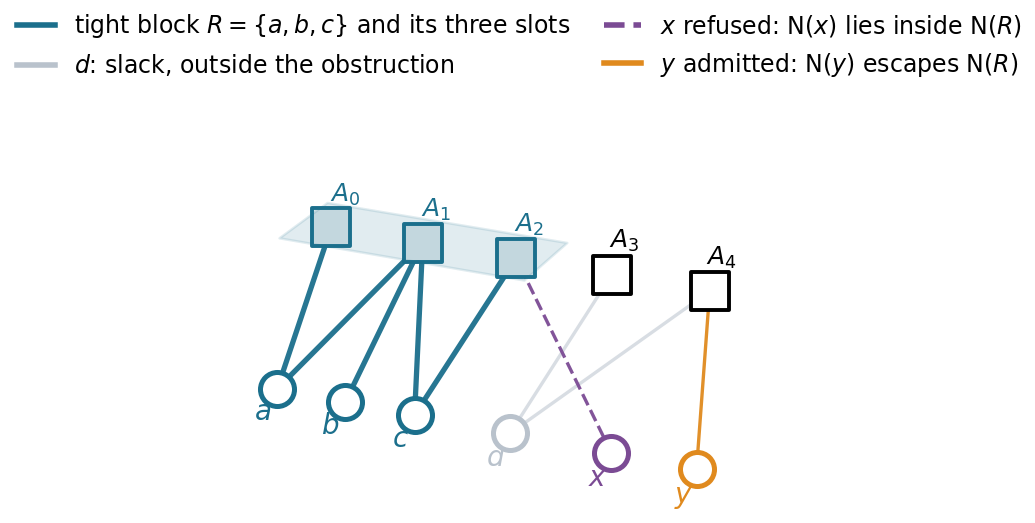
\includegraphics[width=0.86\linewidth]{figures/fig_presentation_3d.png}
\caption{El ejemplo que recorre el artículo, dibujado por
\lean{generate\_obstruction\_figures.py} a partir de los mismos datos que verifica
\lean{check\_canonical\_obstruction.sage}. Cinco conjuntos presentadores sobre $\{a,b,c,d,x,y\}$
dan las ranuras compatibles $\N(a)=\{0,1\}$, $\N(b)=\{1\}$, $\N(c)=\{1,2\}$, $\N(d)=\{3,4\}$,
$\N(x)=\{2\}$, $\N(y)=\{4\}$. El conjunto $I=\{a,b,c,d\}$ es un transversal parcial
($a\!\mapsto\!0$, $b\!\mapsto\!1$, $c\!\mapsto\!2$, $d\!\mapsto\!3$). El plano sombreado es la
vecindad saturada del bloque tight $R=\{a,b,c\}$: tres elementos, tres ranuras, nada de sobra. Es
el muro que rechaza a $x$ y deja pasar a $y$.}
\label{fig:presentation}
\end{figure}

Léase sobre el ejemplo de la Figura~\ref{fig:presentation}: para $I=\{a,b,c,d\}$ todo subconjunto
tiene al menos tantas ranuras como elementos, luego $I$ es factible. Para $\lean{insert}\,x\,I$ el
subconjunto $\{a,b,c,x\}$ tiene cuatro elementos y solo las tres ranuras $\{0,1,2\}$; Hall falla de
inmediato. Lo que importa a continuación es que ese fallo tiene una \emph{forma}. La pregunta que
se pasa adelante es: cuando falla todo intento de inserción, ¿qué comparten esos fallos?

% ---------------------------------------------------------------
\section{Por qué un transversal mayor debe ceder un elemento}\label{sec:q2}

Sean $I,J$ transversales parciales con $|I|<|J|$, y supongamos por reducción al absurdo que ningún
$e\in J\setminus I$ puede insertarse en $I$.

Para cada uno de esos $e$, la caracterización de Hall da un $S\subseteq \lean{insert}\,e\,I$ con
$|\N(S)|<|S|$. Como el propio $I$ cumple Hall, $S$ tiene que contener a $e$ (si no, $S$ sería un
subconjunto violador dentro de $I$); esto es \lean{hall\_violation\_insert\_mem}. Quitemos $e$,
llamemos $R$ al resto, y un breve estrujón de cardinales eleva la desigualdad estricta a cuatro
hechos exactos:
\[
  R\subseteq I,\qquad e\notin R,\qquad |\N(R)|=|R|,\qquad \N(e)\subseteq \N(R).
\]

\begin{recipebox}{El testigo tight (receta)}
Llamemos a $R$ \textbf{tight} cuando satura exactamente sus ranuras compatibles, $|\N(R)|=|R|$
(\lean{IsTight}): no le queda holgura ninguna. Un $R\subseteq I$ tight con $\N(e)\subseteq\N(R)$ es
un \emph{certificado de que $e$ no tiene adónde ir}---toda ranura que $e$ podría usar ya está
comprometida por elementos de $R$, y $R$ no tiene margen para recolocarse. En Lean la extracción es
\lean{exists\_tight\_witness\_of\_not\_insert}: una inserción fallida nunca es un fracaso de
búsqueda sin explicación; siempre devuelve este objeto.
\end{recipebox}

Sobre el ejemplo corriente con $I=\{a,b,c,d\}$, el intento de añadir $x$ devuelve el testigo tight
$R=\{a,b,c\}$: tres elementos llenando las tres ranuras $\{0,1,2\}$, y $\N(x)=\{2\}$ queda dentro
de ellas (Figura~\ref{fig:tight}).

\begin{figure}[htbp]
\centering
\begin{tikzpicture}[font=\small,
  el/.style={circle,draw=tmteal,thick,fill=white,inner sep=1.4pt,minimum size=6.5mm},
  sl/.style={rectangle,draw=black!55,rounded corners=1.5pt,inner sep=2pt,
    minimum width=7.5mm,minimum height=5.5mm,font=\scriptsize}]
  \foreach \i in {0,1,2} \node[sl,fill=tmteal!22] (s\i) at (1.7*\i,1.75) {$A_\i$};
  \foreach \x/\p in {a/0,b/1.7,c/3.4} \node[el] (\x) at (\p,0) {$\x$};
  \node[el,draw=tmplum] (x) at (5.3,0) {$x$};
  \draw[tmteal,line width=1.1pt] (a) -- (s0);
  \draw[tmteal,line width=1.1pt] (a) -- (s1);
  \draw[tmteal,line width=1.1pt] (b) -- (s1);
  \draw[tmteal,line width=1.1pt] (c) -- (s1);
  \draw[tmteal,line width=1.1pt] (c) -- (s2);
  \draw[tmplum,line width=1.2pt,dashed] (x) -- (s2);
  \node[align=left,font=\scriptsize,anchor=west,text=black!70] at (6.1,0.9)
    {$|R|=3=|\N(R)|$: \emph{tight}\\[2pt]
     $\N(x)=\{2\}\subseteq\N(R)$\\[2pt]
     $\Rightarrow$ cuatro elementos,\\tres ranuras: Hall falla};
  \draw[decorate,decoration={brace,amplitude=4pt},tmteal] (-0.5,-0.55) -- (3.9,-0.55)
    node[midway,below=4pt,font=\scriptsize,text=tmteal]{$R=\{a,b,c\}$ es el testigo tight};
\end{tikzpicture}
\caption{Una inserción fallida, explicada y no solo observada. Las tres ranuras sombreadas están
saturadas por $\{a,b,c\}$, y toda ranura que $x$ pudiera ocupar ya está entre ellas. El certificado
es un conjunto, no el rastro de una búsqueda fallida.}
\label{fig:tight}
\end{figure}

Un conjunto tight es local. El aumento necesita una \emph{única} obstrucción que cubra todo
$J\setminus I$ a la vez, y el hecho decisivo es que la propiedad tight sobrevive a la unión. Si
$R,S\subseteq I$ son tight entonces, como $\N(R\cup S)=\N(R)\cup\N(S)$ y
$\N(R\cap S)\subseteq\N(R)\cap\N(S)$,
\keyeq{|\N(R\cup S)|+|\N(R\cap S)| \;\le\; |\N(R)|+|\N(S)| \;=\; |R|+|S| \;=\; |R\cup S|+|R\cap S| ,}
mientras que Hall acota cada término de la izquierda por debajo con su pareja de la derecha. Ambas
desigualdades quedan así forzadas a ser igualdades, y $R\cup S$ es tight (\lean{tight\_union}); la
inducción da la versión para familias finitas, \lean{tight\_biUnion}.

Elijamos ahora un testigo tight $R_e$ para cada $e\in J\setminus I$, pongamos $U=\bigcup_e R_e$ y
apliquemos Hall a $P=(J\setminus I)\cup(U\cap J)\subseteq J$. Su vecindad queda dentro de $\N(U)$, y
$U$ es tight, de modo que la aritmética de cardinales da $|J\setminus I|\le|I\setminus J|$
(\lean{card\_sdiff\_le\_of\_tight\_cover}). Pero para conjuntos finitos $|I|<|J|$ equivale a
$|I\setminus J|<|J\setminus I|$. Contradicción, y el aumento se sigue:
\begin{quote}\ttfamily\small\noindent
theorem partialTransversal\_augmentation\\
\hspace*{1em}(hI : IsPartialTransversal A I) (hJ : IsPartialTransversal A J)\\
\hspace*{1em}(hcard : I.card < J.card) :\\
\hspace*{1em}$\exists$ e $\in$ J \textbackslash\ I, IsPartialTransversal A (insert e I)
\end{quote}
Esta es una prueba del aumento por Hall y conjuntos tight. No implementa emparejamiento máximo ni
búsqueda de caminos de aumento: un teorema de existencia y un algoritmo certificado son entregables
distintos, y aquí solo se reclama el primero.

% ---------------------------------------------------------------
\section{Las tres capas de la prueba}\label{sec:q3}

La dificultad no es el conjunto vacío, ni la restricción, ni el teorema de Hall, que Mathlib ya
proporciona. La verdadera ingeniería de pruebas es el trayecto que va de \emph{varias} inserciones
fallidas a \emph{una} contradicción global. Escrito como un solo argumento es un párrafo; escrito
como un solo bloque de tácticas es ilegible e irreutilizable. Por eso el desarrollo lo separa en
tres capas, y esa separación es la afirmación técnica central del artículo.

\begin{recipebox}{Las tres capas}
\textbf{Capa de emparejamiento.} \lean{compatibleSlots}, \lean{IsPartialTransversal}, la
restricción y \lean{partialTransversal\_iff\_hall}: una interfaz estable entre asignaciones
inyectivas y desigualdades de cardinales. Todo lo que hay por encima habla solo de
cardinales.\\[3pt]
\textbf{Capa de conjuntos tight.} \lean{exists\_tight\_witness\_of\_not\_insert} convierte un fallo
en un objeto; \lean{tight\_union} y \lean{tight\_biUnion} le dan a ese objeto un álgebra. Esta capa
no menciona matroides ni emparejamientos---solo familias de conjuntos y la desigualdad de Hall---, y
justo por eso es reutilizable, y por eso la Sección~\ref{sec:canonical} cuesta casi nada.\\[3pt]
\textbf{Capa de conteo.} \lean{card\_sdiff\_le\_of\_tight\_cover} toma una familia finita de
subconjuntos tight que cubren las ranuras de $J\setminus I$ y devuelve la única desigualdad
$|J\setminus I|\le|I\setminus J|$. El teorema de aumento se limita entonces a elegir un testigo por
cada elemento del subtipo finito $J\setminus I$ e invocarla.
\end{recipebox}

Este es el análogo formal de dibujar la obstrucción antes de contarla. En Lean los detalles son
concretos: los testigos se indexan por un subtipo finito y se eligen con \lean{Exists.choose}; su
unión es un \lean{Finset.biUnion}; una vecindad es ella misma un \lean{biUnion}; y la contradicción
final es aritmética de unión, intersección y diferencia de \lean{Finset} despachada por
\lean{omega}. Ninguno es profundo por separado. Mantenerlos en lemas con nombre propio es lo que
impide que un párrafo combinatorio breve se convierta en una prueba opaca, y es lo que deja la capa
de conjuntos tight disponible para quien la quiera con otro fin.

La afirmación merece decirse sin matices: \emph{la novedad no es que Lean acepte la prueba; es que
la arquitectura de la prueba aísla la obstrucción tight en lemas reutilizables.} Eso es a la vez
una decisión matemática---método de obstrucción en lugar de caminos de aumento---y una decisión de
ingeniería de pruebas, y la Sección~\ref{sec:canonical} es la evidencia de que la decisión fue la
correcta.

% ---------------------------------------------------------------
\section{Empaquetar el matroide}\label{sec:q4}

\lean{IndepMatroid.ofFinset} de Mathlib convierte un predicado de independencia sobre conjuntos
finitos que cumpla los axiomas del vacío, hereditario y de aumento en un matroide finitario. El
desarrollo lo aplica con conjunto base \lean{Set.univ} y predicado \lean{IsPartialTransversal A}:
\begin{quote}\ttfamily\small\noindent
noncomputable def transversalMatroid (A : Fin t $\to$ Finset $\alpha$) : Matroid $\alpha$
\end{quote}
El conjunto base universal es deliberado. Un elemento de $\alpha$ que no aparezca en ningún conjunto
presentador es sencillamente un \emph{lazo}: ningún transversal parcial lo contiene. El teorema
final es por tanto exacto sin restringir antes $\alpha$ a $\bigcup_i A_i$:
\begin{quote}\ttfamily\small\noindent
theorem transversalMatroid\_indep (A : Fin t $\to$ Finset $\alpha$) (I : Finset $\alpha$) :\\
\hspace*{1em}(transversalMatroid A).Indep (I : Set $\alpha$) $\leftrightarrow$ IsPartialTransversal A I
\end{quote}
Este es el teorema del matroide transversal para presentaciones finitas, como un objeto que los
resultados de matroides de Mathlib---rango, clausura, bases, dualidad, menores---pueden consumir
directamente; el Corolario~\ref{cor:closure} ejercita sobre él el operador de clausura, de modo que
la afirmación queda demostrada y no solo enunciada. Se mantiene la distinción entre un teorema
\emph{disponible} y una aplicación \emph{implementada}: la construcción pone la interfaz a
disposición; no implementa aquí ningún optimizador voraz con pesos, ni un oráculo de rango, ni
análisis de complejidad alguno.

% ---------------------------------------------------------------
\section{La obstrucción es canónica}\label{sec:canonical}

A la Sección~\ref{sec:q2} solo le hacía falta que los conjuntos tight fuesen cerrados por
\emph{unión}. Hágasele a la capa de conjuntos tight una pregunta más---¿y la intersección?---y el
mismo estrujón submodular la responde, porque la cadena de desigualdades de arriba fuerza a la vez
la igualdad en \emph{ambos} lados. En Lean esto es un único lema que devuelve una conjunción,
\lean{tight\_union\_and\_inter}; la mitad de la intersección, \lean{tight\_inter}, es la mitad que
el aumento no usa jamás.

\begin{proposition}[Los conjuntos tight forman un retículo; \lean{tight\_union\_and\_inter}]\label{prop:lattice}
Sea $I$ un transversal parcial y sean $R,S\subseteq I$ tight. Entonces $R\cup S$ y $R\cap S$ son
tight. Por tanto los subconjuntos tight de $I$ forman un subretículo del retículo booleano sobre
$I$, que contiene a $\emptyset$.
\end{proposition}

Que los casos de igualdad de la condición de Hall sean cerrados por unión e intersección es teoría
clásica de emparejamientos---es la submodularidad de $\N$, el motor tras la fórmula de defecto de
Ore~\cite{ore} y la descomposición de Dulmage--Mendelsohn~\cite{dm}, y es estándar en Lovász y
Plummer~\cite{lovaszplummer}. No se reclama nada nuevo en la matemática. Lo nuevo es que el
desarrollo por capas lo consigue al precio de añadir un miembro más a la conjunción, y que la
consecuencia de abajo puede entonces siquiera enunciarse.

Como la familia es finita y cerrada por unión, tiene máximo. El desarrollo define
\[
  \lean{tightSubsets}\,A\,I=\{R\in\mathcal P(I) : R \text{ tight}\},\qquad
  \lean{maxTight}\,A\,I=\bigcup \lean{tightSubsets}\,A\,I ,
\]
y prueba que esa unión es ella misma tight (\lean{maxTight\_isTight}, vía \lean{tight\_biUnion}) y
contiene a todo subconjunto tight (\lean{subset\_maxTight}). Es el \emph{máximo}, no meramente un
elemento maximal.

\begin{figure}[htbp]
\centering
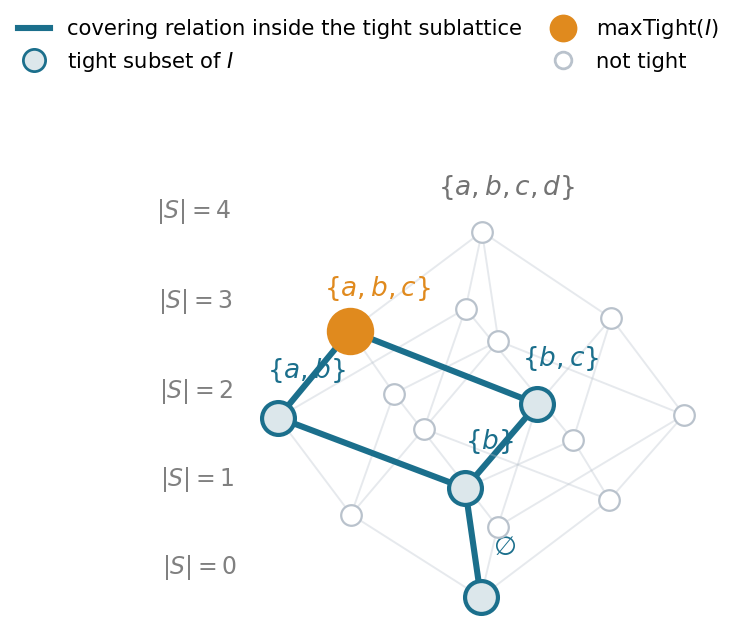
\includegraphics[width=0.62\linewidth]{figures/fig_lattice_3d.png}
\caption{El retículo de subconjuntos tight de $I=\{a,b,c,d\}$, dibujado dentro del retículo booleano
sobre $I$ (la altura es $|S|$); $\lean{maxTight}(I)$ lo corona, y el propio $I$ no es tight. Solo
cinco de los dieciséis subconjuntos son tight, y forman un retículo de verdad, no una cadena:
$\{a,b\}\cap\{b,c\}=\{b\}$ y $\{a,b\}\cup\{b,c\}=\{a,b,c\}$ son ambos tight
(Proposición~\ref{prop:lattice}). La cima, en ámbar, es $\lean{maxTight}(I)=\{a,b,c\}$---un
subconjunto \emph{propio} de $I$, ya que $I$ tiene cuatro elementos y cinco ranuras. Una sola prueba
de contención contra su vecindad decide toda inserción.}
\label{fig:lattice}
\end{figure}

La recompensa es un enunciado de decisión. El lema de existencia de la Sección~\ref{sec:q2} dice que
una inserción fallida \emph{produce} un recubrimiento tight; su recíproco es elemental---si
$R\subseteq I$ es tight, $e\notin R$ y $\N(e)\subseteq\N(R)$, entonces $\lean{insert}\,e\,R$ tiene
$|R|+1$ elementos y solo $|R|$ ranuras, luego Hall falla (\lean{not\_insert\_of\_tight\_cover}).
Necesario y suficiente a la vez; y entonces la monotonía de $\N$ colapsa el existencial sobre el
máximo:

\begin{theorem}[Un solo conjunto decide toda inserción; \lean{insert\_iff\_not\_subset\_maxTight}]
\label{thm:canonical}
Sea $I$ un transversal parcial de $A$ y sea $e\notin I$. Entonces
\[
  \textnormal{\lean{insert}}\,e\,I \ \textnormal{es un transversal parcial}
  \quad\Longleftrightarrow\quad
  \N(e)\ \not\subseteq\ \N\bigl(\textnormal{\lean{maxTight}}\,A\,I\bigr).
\]
\end{theorem}

\noindent El criterio queda enunciado arriba en el vocabulario propio del desarrollo. Puede decirse
en el de Mathlib, y esa es la forma en que se convierte en una afirmación sobre un matroide y no
sobre un predicado hecho a medida:

\begin{corollary}[La obstrucción calcula la clausura; \lean{mem\_closure\_iff\_subset\_maxTight}]
\label{cor:closure}
Con $I$ y $e$ como arriba,
\[
  e\in(\textnormal{\lean{transversalMatroid}}\,A).\textnormal{\lean{closure}}\ I
  \quad\Longleftrightarrow\quad
  \N(e)\subseteq\N\bigl(\textnormal{\lean{maxTight}}\,A\,I\bigr).
\]
\end{corollary}

\noindent \lean{Matroid.closure} es el operador propio de Mathlib, y arrastra consigo su teoría de
planos, conjuntos generadores y rango; el corolario dice que, sobre conjuntos independientes, ese
operador queda decidido por una sola
prueba de contención contra un único conjunto finito canónico---sin búsqueda sobre subconjuntos y
sin recalcular ningún emparejamiento. La prueba son tres líneas: el
\lean{Indep.notMem\_closure\_iff\_of\_notMem} de Mathlib convierte la pertenencia a la clausura en
el fallo de una inserción, \lean{transversalMatroid\_indep} convierte eso en una afirmación sobre
transversales parciales, y el Teorema~\ref{thm:canonical} remata. Con esto queda además saldada la
promesa de la Sección~\ref{sec:q4}: el aparato de la biblioteca sí se aplica al objeto construido, y
aquí se le está aplicando.

Esta es la respuesta a la reserva que deja abierta \emph{Theorem of the Day}---¿cómo sabemos que
nuestros transversales parciales son válidos sin encontrar un emparejamiento al mismo tiempo? Para
un $I$ fijo no hace falta: un solo conjunto tight, calculado una vez, responde toda pregunta
posterior de pertenencia mediante una prueba de contención. En el ejemplo corriente
$\lean{maxTight}=\{a,b,c\}$ con $\N=\{0,1,2\}$, de modo que $\N(x)=\{2\}$ queda dentro y $x$ es
rechazado, mientras que $\N(y)=\{4\}$ queda fuera e $y$ es admitido (Figura~\ref{fig:lattice}). Un
contraste exhaustivo sobre esa presentación---las $56$ transversales parciales y las $180$
decisiones de inserción---coincide con el teorema en todos los casos.

Dos matices honestos. Primero, \lean{maxTight} se define mediante un filtro sobre el conjunto de
partes de $I$, así que la \emph{definición} es exponencial; el teorema certifica la caracterización,
no un procedimiento eficiente, y calcular el máximo conjunto tight de forma eficiente (es una
cuestión de Dulmage--Mendelsohn) se deja a la literatura algorítmica. Segundo, igual que en la
Proposición~\ref{prop:lattice}, la matemática es clásica; la contribución es que sea formal, y que
haya caído de la arquitectura en lugar de exigir un desarrollo nuevo.

% ---------------------------------------------------------------
\begin{figure}[htbp]
\centering
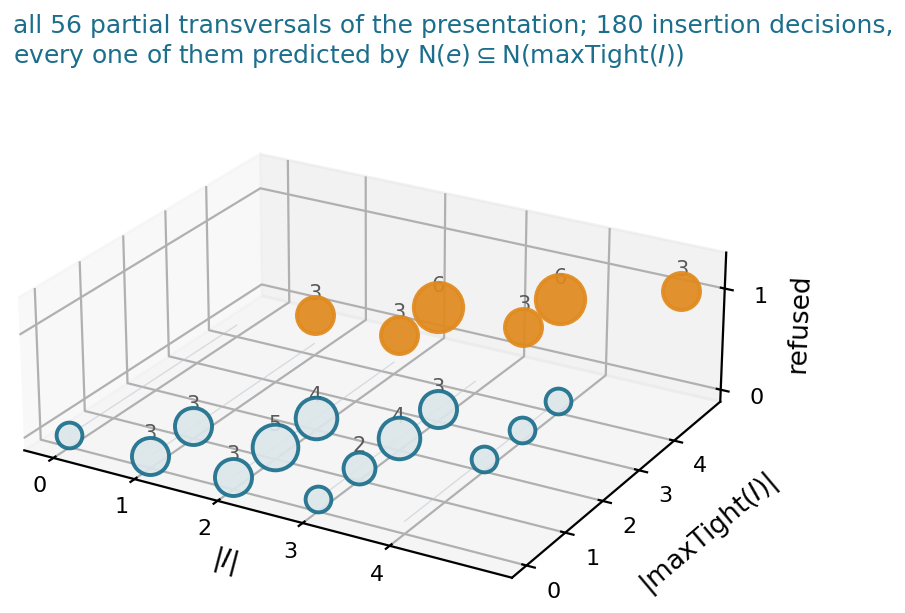
\includegraphics[width=0.72\linewidth]{figures/fig_decision_3d.png}
\caption{El criterio, ejercitado sobre la presentación entera y no sobre un solo ejemplo. Cada
transversal parcial $I$ de la familia corriente se sitúa en
$(|I|,\ |\lean{maxTight}(I)|,\ \#\text{rechazados})$, donde un rechazo significa un elemento fuera
de $I$ que no puede insertarse; el área del marcador cuenta cuántos $I$ comparten posición. El ámbar
marca las posiciones donde la obstrucción canónica muerde de verdad. Las $56$ transversales
parciales y las $180$ decisiones de inserción concuerdan con el Teorema~\ref{thm:canonical}; la
gráfica es la comprobación exhaustiva de \lean{check\_canonical\_obstruction.sage}, no una muestra.}
\label{fig:decision}
\end{figure}

\begin{figure}[htbp]
\centering
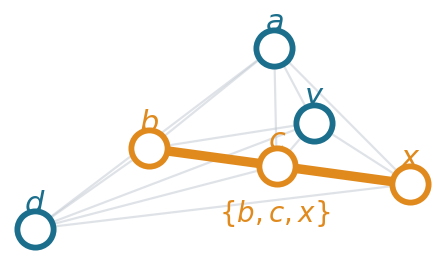
\includegraphics[width=0.74\linewidth]{figures/fig_circuit_3d.png}
\caption{La misma presentación vista como el matroide que define: rango~5 sobre seis elementos,
luego exactamente un circuito. Doce de los trece planos de rango~2 llevan dos puntos; uno lleva
tres, y el dibujo lo respeta colocando $b$, $c$ y $x$ sobre una recta. Esa recta \emph{es} el
violador de Hall, $\N(\{b,c,x\})=\{A_1,A_2\}$---tres puntos compitiendo por dos ranuras---y todo
rechazo en cualquier punto de esta presentación se remonta a ella. El circuito y la obstrucción
tight son el mismo fenómeno leído desde lados opuestos: un conjunto tight es lo que queda de un
circuito al quitarle uno de sus elementos.}
\label{fig:circuit}
\end{figure}

\section{Las piezas}\label{sec:blocks}

La Tabla~\ref{tab:results} reúne los resultados que sostienen el edificio; la
Tabla~\ref{tab:metrics} mide el desarrollo. La cadena de dependencias es corta: la capa de
emparejamiento da la equivalencia de Hall; la equivalencia de Hall da el testigo tight;
\lean{tight\_union\_and\_inter} dota a los conjuntos tight de un álgebra; la capa de conteo
convierte un recubrimiento en una sola desigualdad; y el retículo da la obstrucción canónica.

\begin{table}[H]
  \centering\footnotesize
  \arrayrulecolor{tmteal}
  \begin{tabular}{@{}llc@{}}
    \toprule
    \rowcolor{tmteal}
    \textcolor{white}{\textbf{Nombre Lean}} & \textcolor{white}{\textbf{Enunciado}} & \textcolor{white}{\textbf{Estado}} \\
    \midrule
    \multicolumn{3}{@{}l}{\emph{\lean{TransversalMatroid.lean}} --- la construcción} \\
    \rowcolor{tmband}
    \lean{partialTransversal\_empty} & $\emptyset$ es un transversal parcial & probado \\
    \lean{partialTransversal\_subset} & restricción de un emparejamiento (herencia) & probado \\
    \rowcolor{tmband}
    \lean{partialTransversal\_iff\_hall} & factible $\iff$ $|S|\le|\N(S)|$ en todo $S\subseteq I$ & probado \\
    \lean{hall\_violation\_insert\_mem} & un subconjunto violador contiene a $e$ & probado \\
    \rowcolor{tmband}
    \lean{exists\_tight\_witness\_of\_not\_insert} & inserción fallida $\Rightarrow$ testigo tight & probado \\
    \lean{tight\_union}, \lean{tight\_biUnion} & lo tight sobrevive a la unión finita & probado \\
    \rowcolor{tmband}
    \lean{card\_sdiff\_le\_of\_tight\_cover} & $|J\setminus I|\le|I\setminus J|$ desde un recubrimiento & probado \\
    \lean{partialTransversal\_augmentation} & el axioma de intercambio & probado \\
    \rowcolor{tmband}
    \lean{transversalMatroid\_indep} & \lean{Indep} $\iff$ transversal parcial & probado \\
    \midrule
    \multicolumn{3}{@{}l}{\emph{\lean{TransversalObstruction.lean}} --- la obstrucción canónica} \\
    \lean{tight\_union\_and\_inter} & los conjuntos tight forman un retículo & probado \\
    \rowcolor{tmband}
    \lean{maxTight\_isTight} & la cima del retículo es tight & probado \\
    \lean{subset\_maxTight} & es el máximo, no solo maximal & probado \\
    \rowcolor{tmband}
    \lean{not\_insert\_of\_tight\_cover} & un recubrimiento tight bloquea la inserción & probado \\
    \lean{not\_insert\_iff\_exists\_tight} & fallo $\iff$ algún recubrimiento tight & probado \\
    \rowcolor{tmband}
    \lean{insert\_iff\_not\_subset\_maxTight} & un conjunto decide toda inserción & probado \\
    \rowcolor{tmband}
    \lean{mem\_closure\_iff\_subset\_maxTight} & calcula \lean{Matroid.closure} & probado \\
    \bottomrule
  \end{tabular}
  \arrayrulecolor{black}
  \caption{El desarrollo, entero sin \lean{sorry}, en Lean~4 / Mathlib. \lean{\#print axioms} sobre
  \lean{partialTransversal\_augmentation}, \lean{transversalMatroid\_indep},
  \lean{tight\_union\_and\_inter}, \lean{maxTight\_isTight},
  \lean{insert\_iff\_not\_subset\_maxTight} y \lean{mem\_closure\_iff\_subset\_maxTight}
  devuelve únicamente \lean{propext}, \lean{Classical.choice} y \lean{Quot.sound}.}
  \label{tab:results}
\end{table}

\begin{table}[H]
  \centering\footnotesize
  \arrayrulecolor{tmteal}
  \begin{tabularx}{0.96\linewidth}{@{}>{\raggedright\arraybackslash}p{0.36\linewidth}X@{}}
    \toprule
    \rowcolor{tmteal}
    \textcolor{white}{\textbf{Magnitud}} & \textcolor{white}{\textbf{Valor}} \\
    \midrule
    \rowcolor{tmband}
    Líneas: construcción $/$ obstrucción & $400\,/\,245$ \\
    Teoremas $+$ definiciones & $15{+}4$ $/$ $19{+}5$ \\
    \rowcolor{tmband}
    Importaciones directas de Mathlib & $3$: \lean{Combinatorics.Hall.Basic},
      \lean{Matroid.IndepAxioms}, \lean{Matroid.Closure} \\
    \lean{sorry} / \lean{admit} / \lean{native\_decide} & $0$ \\
    \rowcolor{tmband}
    Axiomas más allá del núcleo de Lean & $0$: solo \lean{propext}, \lean{Classical.choice},
      \lean{Quot.sound} \\
    Compilación & \lean{lake build}
      \lean{Theorems.TransversalObstruction} --- $1164$ tareas, salida~$0$ \\
    \rowcolor{tmband}
    Compilación, Mathlib en caliente & ${\approx}\,4.7$\,s (módulo de la obstrucción) \\
    Cadena de herramientas & Lean~4 \lean{v4.32.0}; Mathlib \lean{84fdd0bf} (2026-07-15) \\
    \rowcolor{tmband}
    Contraste Sage & $56$ transversales parciales, $180$ decisiones de inserción \\
    \bottomrule
  \end{tabularx}
  \arrayrulecolor{black}
  \caption{El desarrollo, medido. La huella es deliberadamente ligera: dos importaciones de
  Mathlib y nada de álgebra pesada, porque el argumento es conteo elemental una vez separadas las
  capas. La fila de Sage~\cite{sage} es un contraste ejecutable del ejemplo corriente, no evidencia
  de los teoremas; esa evidencia es el núcleo de Lean.}
  \label{tab:metrics}
\end{table}

% ---------------------------------------------------------------
\section{El límite de la contribución}\label{sec:boundary}

\emph{Qué está probado.} El teorema del matroide transversal para presentaciones finitas
\lean{A : Fin t $\to$ Finset $\alpha$}: los transversales parciales cumplen los tres axiomas de
conjunto independiente y son exactamente los conjuntos finitos independientes de
\lean{transversalMatroid A}; más el retículo de conjuntos tight, el subconjunto tight máximo y el
criterio de inserción del Teorema~\ref{thm:canonical}. Todo sin \lean{sorry}, con el perfil de
axiomas de arriba.

\emph{Solo presentaciones finitas.} La familia es finita y cada $A_i$ es finito. El tipo ambiente
$\alpha$ no tiene por qué ser finito, pero el desarrollo caracteriza los conjuntos independientes
\emph{finitos} y usa la construcción finitaria de Mathlib. La versión infinita---la que Mirsky y
Perfect probaron también~\cite{mirskyperfect}---no queda cubierta.

\emph{Ninguna afirmación algorítmica.} La prueba selecciona testigos tight con elección clásica.
Prueba el aumento; no implementa búsqueda de caminos de aumento, ni emparejamiento máximo, ni cota
alguna. \lean{maxTight} se define por un filtro sobre el conjunto de partes y no es un
procedimiento eficiente.

\emph{La matemática es clásica.} Edmonds--Fulkerson y Mirsky--Perfect probaron el teorema; el
método de conjuntos tight es teoría estándar de transversales y
emparejamientos~\cite{ore,dm,lovaszplummer,welsh,oxley}. Lo que se ofrece aquí es la formalización,
su arquitectura, y el empaquetado de la obstrucción como objeto canónico.

\emph{Autoría.} La formalización se llevó a cabo en interacción estrecha con un asistente de IA
(Claude, Anthropic): la elección del objetivo, la arquitectura de la prueba, los enunciados y las
afirmaciones de alcance y novedad son míos; el asistente redactó e iteró buena parte del Lean bajo
esa dirección. Esto no afecta a la validez---una prueba se acepta solo cuando el núcleo de Lean la
verifica, cosa que hace, con el perfil de axiomas indicado arriba---, pero se declara sin rodeos por
atribución.

\emph{Frontera de confianza.} Los tres axiomas indicados describen los teoremas tal como los
verifica el entorno de Lean actual. No son una afirmación de haber eliminado el núcleo de Lean, ni
el compilador, ni el hardware, del círculo de confianza.

% ---------------------------------------------------------------
\section{Prioridad: qué se buscó, cuándo, y qué la refutaría}\label{sec:priority}

Las afirmaciones del tipo ``esto no estaba formalizado'' se degradan. Son ciertas de un momento, de
un conjunto de bibliotecas y de un conjunto de consultas, y las tres cosas cambian. Esta sección
fija las tres para que quien lea dentro de unos años pueda \emph{comprobar} la afirmación en lugar
de confiar en ella y, si ha dejado de ser cierta, pueda decir exactamente cuándo dejó de serlo.

{\sloppy\emph{Qué se afirma.} Dos cosas, y nada más allá de ellas. (i) Hasta donde sé, el matroide
\lean{transversalMatroid} es el primero de Mathlib construido a partir de una presentación
combinatoria y no por una construcción trivial o dual. (ii) Hasta donde sé, el teorema del matroide
transversal no había sido formalizado en ningún asistente de pruebas antes de este
desarrollo.\par} Ambas son afirmaciones sobre la \emph{formalización}, nunca sobre la matemática,
que es de Edmonds--Fulkerson y de Mirsky--Perfect y tiene sesenta años.

\emph{Qué no se afirma.} Ninguna prioridad sobre enunciado matemático alguno de este artículo.
Ninguna afirmación de que el área circundante esté sin formalizar---no lo está: el AFP contiene
algoritmos verificados para matroides y greedoides, incluido el emparejamiento bipartito
máximo~\cite{itp2025}, y Mathlib contiene una teoría estructural de matroides sustancial. Y ninguna
afirmación sobre trabajo que no pude leer, incluidos desarrollos inéditos, repositorios privados y
formalizaciones archivadas bajo otro nombre.

\emph{Qué se buscó exactamente, y cuándo.} Todo lo siguiente, en julio de 2026.

\begin{itemize}\itemsep2pt
\item \textbf{Mathlib}, revisión \lean{84fdd0bf} (15-07-2026), cadena de herramientas
\lean{v4.32.0}: una búsqueda de texto sin distinción de mayúsculas de \emph{transversal} sobre todo
\lean{Mathlib/}, que devuelve \lean{Combinatorics/Hall/Basic.lean} (solo en prosa) y nueve ficheros
de teoría de grupos (\lean{GroupTheory/Complement}, \lean{CosetCover}, \lean{Schreier},
\lean{SchurZassenhaus}, \lean{Transfer} y otros), y ninguna aparición de \emph{transversal matroid};
más una lectura de todas las declaraciones de \lean{Combinatorics/Matroid/Constructions.lean}, que
define exactamente \lean{emptyOn}, \lean{loopyOn}, \lean{freeOn} y \lean{uniqueBaseOn}.
\item \textbf{Isabelle/AFP}: el índice temático de combinatoria, y búsquedas de \emph{transversal
matroid}, \emph{transversal}, \emph{matroid} y \emph{marriage}. Encontrado: \emph{Matroids}
(Keinholz, 2018)~\cite{afpmatroids}, \emph{Hall's Marriage Theorem} (Jiang y Nipkow,
2010)~\cite{afphall}, y el trabajo de ITP~2025 sobre algoritmos de matroides y
greedoides~\cite{itp2025}. Ninguna entrada de matroide transversal localizada.
\item \textbf{Mizar, Coq/\lean{mathcomp}, HOL~Light}: búsquedas con los mismos términos. Se
localizaron teoremas vecinos sobre conjuntos finitos en Coq~\cite{coqdilworth}; no se localizó
ninguna formalización del matroide transversal en ninguno de los tres. Esta es la pata más débil de
la auditoría: se apoya en búsqueda pública y no en la lectura del índice de cada biblioteca, y
consideraría que un aviso por aquí tiene más probabilidad de acertar que uno dirigido a Mathlib o
al AFP.
\end{itemize}

\emph{Qué la refutaría.} Un único localizador---biblioteca, nombre de la entrada, fichero,
fecha---de una formalización del teorema del matroide transversal, o de cualquier matroide de
Mathlib construido a partir de datos combinatorios anterior a la revisión \lean{84fdd0bf}, refuta
de plano la afirmación correspondiente. Nada más en este artículo depende de ninguna de las dos: el
desarrollo en Lean, el perfil de axiomas, el retículo de conjuntos tight y el
Teorema~\ref{thm:canonical} se sostienen o caen por el núcleo, no por la prioridad. Agradecería que
se me enviara ese localizador, y lo dejaría consignado.

% ---------------------------------------------------------------
\section{Conclusión}\label{sec:conclusion}

He formalizado el teorema del matroide transversal para presentaciones finitas en Lean~4 sobre
Mathlib, y lo he empaquetado como objeto matroide, \lean{transversalMatroid A}, cuyos conjuntos
finitos independientes identifica exactamente \lean{transversalMatroid\_indep}. Hasta donde
sé---frente a las búsquedas fechadas y detalladas en la Sección~\ref{sec:priority}, y con los
límites que allí se declaran---es el primer matroide de Mathlib construido a partir de datos
combinatorios y no de una construcción trivial o dual.

He probado el aumento---el único axioma que la definición no regala---por el método de obstrucción
de Hall y no por caminos de aumento, y he organizado esa prueba en tres capas independientes: una
interfaz de emparejamiento sobre el teorema de Hall finito de Mathlib, una capa de conjuntos tight
con álgebra propia, y una capa de conteo que convierte un recubrimiento de conjuntos tight en una
única contradicción de cardinales. Cada paso es un lema con nombre propio y reutilizable por
separado.

{\sloppy El objeto resultante se integra directamente con Mathlib. Se produce mediante
\lean{IndepMatroid.ofFinset}, de modo que la teoría de rango, clausura, bases, dualidad y menores de
la biblioteca se le aplica sin trabajo adicional, y el conjunto base se toma universal, de manera
que los elementos ajenos a todo conjunto presentador son lazos y la caracterización es exacta. Esa
integración se ejercita, no se declara: el Corolario~\ref{cor:closure} identifica la propia
\lean{Matroid.closure} de Mathlib, sobre conjuntos independientes, con una sola prueba de
contención contra \lean{maxTight}.\par}

La arquitectura se pagó sola. Los conjuntos tight son cerrados por intersección además de por
unión, luego forman un retículo; todo transversal parcial tiene un subconjunto tight máximo; y una
sola prueba de contención contra su vecindad decide toda inserción
(Teorema~\ref{thm:canonical}). La obstrucción no es un incidente de una búsqueda fallida, sino un
invariante canónico del par (presentación, conjunto independiente).

\emph{Trabajo futuro}, en el orden en que lo intentaría: extraer un procedimiento ejecutable que
devuelva o bien un aumento o bien el certificado tight, y conectarlo con los algoritmos de
emparejamiento verificados de la literatura de Isabelle~\cite{itp2025}; llevar el
Corolario~\ref{cor:closure} hasta el rango, donde el valor debería ser la fórmula de defecto de
Ore
$r(X)=\min_{S\subseteq X}\bigl(|X\setminus S|+|\N(S)|\bigr)$~\cite{ore}---verificada exhaustivamente sobre la
presentación corriente por \lean{check\_canonical\_obstruction.sage} y \emph{no} formalizada, que es
justo por lo que es trabajo futuro y no un resultado; elevar la construcción a familias indexadas
infinitas, siguiendo a Mirsky y Perfect y la propia vía de compacidad de Mathlib para Hall; y
promover la capa de conjuntos tight a contribución autónoma de Mathlib, ya que trata de sistemas
finitos de conjuntos y no menciona matroide alguno.

% ---------------------------------------------------------------
\section{Reflexiones}\label{sec:reflections}

Formalizar un teorema de mediados de los sesenta no es, en sí, interesante. Lo que enseñó el
ejercicio sí lo es, y estas siete observaciones son el residuo.

\paragraph{1. Un teorema no es el mismo objeto que la razón por la que es cierto.}
El teorema del matroide transversal afirma que algo \emph{siempre puede} hacerse: un transversal
mayor siempre cede un elemento. La prueba, en cambio, procede enteramente estudiando lo que
\emph{no puede} hacerse. Formalizar sacó esa asimetría a la luz, porque un núcleo no acepta ``se ve
que algún elemento tiene que servir''; exige una construcción, y la única construcción disponible es
la del obstáculo. El objeto negativo resultó ser el más rico---lleva adjuntos un retículo, un máximo
y un procedimiento de decisión---, mientras que el enunciado positivo no tiene nada de eso. Merece
enunciarse como heurística de trabajo: cuando un teorema afirma que cierta elección existe, el
contenido formalizable suele vivir en la clasificación de las razones por las que podría no existir.

\paragraph{2. Las bibliotecas formales son ricas en teoría y pobres en ejemplos.}
Mathlib sabe calcular el dual, los menores, el rango y la clausura de un matroide, y en la revisión
\lean{84fdd0bf} no tenía prácticamente ningún matroide al que aplicárselo. El desequilibrio es
estructural y no accidental: la teoría se enuncia una vez y se reutiliza, mientras que cada familia
de ejemplos---gráficos, lineales, transversales---cuesta su propia construcción, y las
construcciones se hacen las últimas. El mismo patrón se ve en cualquier biblioteca grande. Si uno
quiere ser útil a una biblioteca formal, y no solo estar presente en ella, construir un ejemplo que
su teoría existente pueda masticar puede valer más que otro teorema sobre objetos que nadie ha
instanciado.

\paragraph{3. Las capas no fueron pulcritud: fueron adonde se fue la matemática.}
Partir la prueba en una capa de emparejamiento, una de conjuntos tight y una de conteo se hizo por
legibilidad. Resultó ser el acto sustantivo. Una vez que los conjuntos tight tuvieron capa propia,
preguntar si eran cerrados por intersección era una pregunta natural cuya respuesta costaba un
miembro más en la conjunción, y el Teorema~\ref{thm:canonical} vino detrás. Si la prueba del aumento
se hubiera escrito como un solo argumento---como está en los libros de texto, y como habría salido
en un primer intento en Lean---, el retículo habría quedado invisible, porque no habría habido
objeto al que hacerle la pregunta. Ingeniería de pruebas y descubrimiento matemático fueron, aquí,
la misma actividad.

\paragraph{4. Un certificado vale más que una búsqueda.}
Un algoritmo de caminos de aumento responde a ``¿puede insertarse $e$?'' ejecutándose, y vuelve a
responder ejecutándose otra vez. El conjunto tight responde una sola vez y queda reutilizable para
toda pregunta posterior sobre el mismo $I$. La reserva que la propia página de \emph{Theorem of the
Day} pone a este teorema---que la selección voraz ``deja abierta la cuestión de cómo sabemos que
nuestros transversales parciales son válidos si no encontramos un emparejamiento al mismo
tiempo''---es precisamente una queja sobre la búsqueda, y la obstrucción canónica es la respuesta.
Que un rechazo venga con su razón adjunta es un principio de diseño que generaliza mucho más allá de
los matroides.

\paragraph{5. Clásico no quiere decir disponible.}
Todos los ingredientes matemáticos de aquí tienen décadas: Hall en 1935, el teorema mismo en
1965--67, y la submodularidad de la función de vecindad es más antigua que ambos. Y sin embargo
ningún asistente de pruebas tenía el enunciado, y la razón no es la dificultad. Es que los
resultados clásicos se ensamblan a partir de prerrequisitos que las bibliotecas adquieren en un
orden distinto al de los libros de texto, de modo que el coste marginal de un teorema dentro de una
biblioteca tiene poco que ver con su coste marginal sobre el papel. Esto corta por los dos lados:
explica por qué algunos teoremas célebres siguen sin formalizar, y significa que un resultado
clásico modesto puede ser aun así una contribución real a una biblioteca.

\paragraph{6. La definición correcta cuesta menos que la prueba ingeniosa.}
Definir \lean{IsPartialTransversal} como la no vacuidad del \lean{hallMatchingsOn} de Mathlib, y no
como un predicado a medida, fue la única decisión que hizo corto el desarrollo. Compró de golpe la
dirección recíproca de Hall, y convirtió todo lema posterior en una afirmación sobre cardinales en
lugar de sobre funciones. La tentación contraria---definir un predicado cómodo y luego probar que
equivale al de la biblioteca---habría añadido una capa de traducción a cada prueba. Cuando una
biblioteca ya habla de tu objeto, casi siempre sale más barato hablar su dialecto que introducir el
propio.

\paragraph{7. Qué cambió el asistente, y qué no.}
Este desarrollo se escribió en interacción estrecha con un asistente de IA, y conviene ser preciso
sobre el efecto. Comprimió la distancia mecánica entre una idea y una prueba verificada, de modo que
en una tarde cupieron más variantes arquitectónicas de las que habrían cabido en una semana---y fue
esa iteración barata, y no ninguna intuición concreta, la que sacó a la superficie la mitad de la
intersección de la Proposición~\ref{prop:lattice}. Lo que no cambió es el criterio de verdad. El
núcleo aceptó o rechazó, el informe de axiomas lo genera la máquina, y las declaraciones de alcance
de la Sección~\ref{sec:boundary} son afirmaciones de las que responde una persona. Una forma más
rápida de probar cosas no baja el listón; si acaso, hace más importante enunciarlo de forma
explícita.

% ---------------------------------------------------------------
\section{Cabos sueltos}\label{sec:questions}

Cuatro preguntas que el trabajo plantea y no resuelve.

\begin{enumerate}\itemsep3pt
\item \emph{Del testigo al algoritmo.} El testigo tight ya explica un rechazo. ¿Puede convertirse la
prueba de existencia en un procedimiento verificado que devuelva o bien un transversal mayor o bien
un certificado comprobable de vecindad saturada---y hace el máximo conjunto tight, obtenido de una
descomposición de Dulmage--Mendelsohn, que ese procedimiento sea polinómico con el certificado de
regalo?
\item \emph{Qué finitud hace falta de verdad.} La prueba usa la finitud en tres sitios distintos:
para elegir testigos, para tomar una unión finita y para hacer aritmética de cardinales. ¿Cuál de
los tres sobrevive a presentaciones infinitas, y basta el argumento de compacidad de Mathlib para
Hall para cargar con el resto?
\item \emph{¿Pertenece a Mathlib la capa de conjuntos tight?} \lean{tight\_union\_and\_inter} y
\lean{tight\_biUnion} no dicen nada sobre matroides. Son lemas sobre un sistema finito de conjuntos
y el caso de igualdad de la condición de Hall. Eso es un enunciado con forma de Mathlib buscando
casa.
\item \emph{Una obstrucción, tres caras.} El retículo de conjuntos tight es el mismo fenómeno que la
descomposición de Dulmage--Mendelsohn de un grafo bipartito y que el violador maximal canónico en
optimización submodular. ¿Existe una única noción en Lean---una función submodular y su retículo de
igualdad---que subsuma las tres, con el caso transversal como instancia? Esa es la cuenta del collar
que más me gustaría seguir enhebrando.
\end{enumerate}

% ---------------------------------------------------------------
\section*{Reproducir}

\begin{verbatim}
lake build Theorems.TransversalMatroid      # la construccion
lake build Theorems.TransversalObstruction  # la obstruccion canonica
lake env lean formalizations/transversal-matroid/lean/
              Theorems/AxiomReport.lean     # el informe de confianza
python formalizations/transversal-matroid/sage/check_canonical_obstruction.sage
\end{verbatim}
{\sloppy Lean~4, cadena de herramientas \lean{leanprover/lean4:v4.32.0}, sobre Mathlib en la
revisión
\lean{84fdd0bf} (2026-07-15):
\begin{center}
\url{https://github.com/leanprover-community/mathlib4}\\[2pt]
fijada en
\href{https://github.com/leanprover-community/mathlib4/commit/84fdd0bfb8e85237f54b9617cca79c6198d40a75}%
{\lean{84fdd0bfb8e85237f54b9617cca79c6198d40a75}}
\end{center}
Los dos módulos de Mathlib sobre los que se apoya este desarrollo, en esa revisión, son
\href{https://github.com/leanprover-community/mathlib4/blob/84fdd0bfb8e85237f54b9617cca79c6198d40a75/Mathlib/Combinatorics/Hall/Basic.lean}%
{\lean{Combinatorics/Hall/Basic.lean}} and
\href{https://github.com/leanprover-community/mathlib4/blob/84fdd0bfb8e85237f54b9617cca79c6198d40a75/Mathlib/Combinatorics/Matroid/IndepAxioms.lean}%
{\lean{Combinatorics/Matroid/IndepAxioms.lean}}; y el módulo de construcciones cuyo contenido
reporta la Sección~\ref{sec:priority} es
\href{https://github.com/leanprover-community/mathlib4/blob/84fdd0bfb8e85237f54b9617cca79c6198d40a75/Mathlib/Combinatorics/Matroid/Constructions.lean}%
{\lean{Combinatorics/Matroid/Constructions.lean}}. Toda afirmación de ausencia de este artículo es
comprobable contra esas URL exactas, y lo sigue siendo después de que Mathlib avance. Para
reproducirlo en otra máquina, apúntese \lean{lakefile.lean} a una Mathlib compilada con la misma
cadena de herramientas; la ruta local usada aquí está registrada en
\lean{MATHLIB\_ENVIRONMENT.md}.\par}

{\sloppy Las fuentes en Lean, el informe de axiomas generado, el contraste exhaustivo en SageMath y
el generador determinista de figuras están archivados junto con las demás formalizaciones de esta
serie~\cite{neumann,gglean,newtonlean} en
\url{https://github.com/karlesmarin/godsil-gutman-lean}. Ambos ficheros Lean están sin
\lean{sorry}, y \lean{\#print axioms} sobre los seis teoremas listados en la
Tabla~\ref{tab:results} devuelve únicamente \lean{propext}, \lean{Classical.choice} y
\lean{Quot.sound}. El registro de verificación a nivel de fuente es \lean{VERIFICATION.md}; y el
ejemplo corriente de cada figura se rederiva de forma exhaustiva---las $56$ transversales parciales
y las $180$ decisiones de inserción---mediante \lean{check\_canonical\_obstruction.sage} antes de
dibujar figura alguna.\par}

\begin{thebibliography}{99}\small
\bibitem{hall} P.~Hall, On representatives of subsets, \emph{J.~London Math.\ Soc.} \textbf{10}
(1935), 26--30. \url{https://doi.org/10.1112/jlms/s1-10.37.26}.
\bibitem{edmondsfulkerson} J.~Edmonds, D.~R.~Fulkerson, Transversals and matroid partition,
\emph{J.~Res.\ Nat.\ Bur.\ Standards Sect.~B} \textbf{69B} (1965), 147--153.
\bibitem{mirskyperfect} L.~Mirsky, H.~Perfect, Applications of the notion of independence to
problems of combinatorial analysis, \emph{J.~Combin.\ Theory} \textbf{2} (1967), 327--357.
\bibitem{perfect} H.~Perfect, Applications of Menger's graph theorem, \emph{J.~Math.\ Anal.\
Appl.} \textbf{22} (1968), 96--111. \url{https://doi.org/10.1016/0022-247X(68)90163-7}.
\bibitem{totd} R.~Whitty, The Transversal Matroid Theorem, \emph{Theorem of the Day},
\url{https://www.theoremoftheday.org/CombinatorialTheory/Transversal/TotDTransversal.pdf}
(attribution: ``proved in the mid-1960s by Jack Edmonds and Delbert Ray Fulkerson in the USA and,
independently (and also in an infinite version) by Leon Mirsky and Hazel Perfect at Sheffield
University in the UK'').
\bibitem{rado} R.~Rado, A theorem on independence relations, \emph{Quart.\ J.~Math.\ Oxford Ser.}
\textbf{13} (1942), 83--89 (el criterio de Hall generalizado a matroides).
\bibitem{perfectthesis} H.~Perfect, \emph{Studies in Transversal Theory with Particular Reference
to Independence Structures and Graphs}, tesis doctoral, University of London, 1969.
\bibitem{perfectmirsky} H.~Perfect, L.~Mirsky, Spectral properties of doubly-stochastic matrices,
\emph{Monatsh.\ Math.} \textbf{69} (1965), 35--57. \url{https://doi.org/10.1007/BF01313442} (el
origen de la conjetura de Perfect--Mirsky).
\bibitem{oxleywelsh} J.~Oxley, The contributions of Dominic Welsh to matroid theory,
\url{https://www.math.lsu.edu/~oxley/dominic.pdf} (sobre las escuelas de Oxford y Sheffield, y sobre
el congreso de Edmonds de 1965 en el National Bureau of Standards).
\bibitem{whitney} H.~Whitney, On the abstract properties of linear dependence, \emph{Amer.\ J.\
Math.} \textbf{57} (1935), 509--533 (el artículo que da nombre al matroide, publicado el mismo año que el de
Hall).
\bibitem{farroxley} G.~Farr, J.~Oxley, The contributions of W.~T.~Tutte to matroid theory,
\url{https://www.math.lsu.edu/~oxley/Tutte_farrox5.pdf} (sobre el letargo de la teoría de matroides tras
1935 y su renacer con los artículos de Tutte de 1958--59).
\bibitem{bryantperfect} V.~Bryant, H.~Perfect, \emph{Independence Theory in Combinatorics: An
Introductory Account with Applications to Graphs and Transversals}, Chapman and Hall, 1980.
\bibitem{ore} O.~Ore, Graphs and matching theorems, \emph{Duke Math.\ J.} \textbf{22} (1955),
625--639 (la forma de defecto del teorema de Hall).
\bibitem{dm} A.~L.~Dulmage, N.~S.~Mendelsohn, Coverings of bipartite graphs, \emph{Canad.\ J.\
Math.} \textbf{10} (1958), 517--534.
\bibitem{lovaszplummer} L.~Lov\'asz, M.~D.~Plummer, \emph{Matching Theory}, North-Holland, 1986.
\bibitem{welsh} D.~J.~A.~Welsh, \emph{Matroid Theory}, Academic Press, 1976.
\bibitem{oxley} J.~G.~Oxley, \emph{Matroid Theory}, 2nd ed., Oxford University Press, 2011.
\bibitem{ingleton} A.~W.~Ingleton, Transversal matroids and related structures, in \emph{Higher
Combinatorics}, NATO ASI Series~C \textbf{31}, Reidel, 1977, 117--131.
\bibitem{gusakov} A.~Gusakov, B.~Mehta, K.~A.~Miller, Formalizing Hall's marriage theorem in Lean,
2021. \url{https://arxiv.org/abs/2101.00127} (el desarrollo de Mathlib que se usa aquí:
\lean{Mathlib.Combinatorics.Hall.Basic}).
\bibitem{afphall} D.~Jiang, T.~Nipkow, Hall's Marriage Theorem, \emph{Archive of Formal Proofs}
(2010). \url{https://isa-afp.org/entries/Marriage.html}.
\bibitem{afpmatroids} J.~Keinholz, Matroids, \emph{Archive of Formal Proofs} (2018).
\url{https://isa-afp.org/entries/Matroids.html}.
\bibitem{coqdilworth} A.~Singh, R.~Natarajan, Fully mechanized proofs of Dilworth's theorem and
Mirsky's theorem, 2017. \url{https://arxiv.org/abs/1703.06133} (Coq; teoremas vecinos sobre conjuntos
finitos).
\bibitem{itp2025} \emph{A Formal Analysis of Algorithms for Matroids and Greedoids},
\emph{Interactive Theorem Proving (ITP 2025)}, LIPIcs, Schloss Dagstuhl.
\url{https://drops.dagstuhl.de/entities/document/10.4230/LIPIcs.ITP.2025.2} (incluye emparejamiento bipartito
máximo ejecutable).
\bibitem{binarymatroids} \emph{Formalizing the Excluded Minor Characterization of Binary Matroids
in the Lean Theorem Prover}, University of Waterloo, 2023.
\url{https://uwspace.uwaterloo.ca/items/d35d17be-485d-4f60-8696-4dce7ae907bb}.
\bibitem{seymour} \emph{Composition Direction of Seymour's Theorem for Regular Matroids ---
Formally Verified}, 2025. \url{https://arxiv.org/abs/2509.20539}.
\bibitem{mathlib} The mathlib Community, The Lean mathematical library, in \emph{Certified
Programs and Proofs (CPP 2020)}, ACM, 2020, 367--381.
\url{https://doi.org/10.1145/3372885.3373824}. Repository:
\url{https://github.com/leanprover-community/mathlib4}; este trabajo se verifica contra la revisión
\lean{84fdd0bfb8e85237f54b9617cca79c6198d40a75} (2026-07-15).
\bibitem{lean4} L.~de Moura, S.~Ullrich, The Lean~4 theorem prover and programming language, in
\emph{Automated Deduction (CADE~28)}, LNCS \textbf{12699}, Springer, 2021, 625--635.
\url{https://doi.org/10.1007/978-3-030-79876-5_37}. Repository:
\url{https://github.com/leanprover-community/lean4}.
\bibitem{sage} The Sage Developers, \emph{SageMath, the Sage Mathematics Software System}.
\url{https://www.sagemath.org}.
% --- this string of formalizations ---
\bibitem{neumann} C.~Mar\'in, \emph{When Separation Fails, a Canon Appears: one counting identity
behind separation, synchronization and symmetry-breaking in permutation groups, formalized in
Lean~4}, Zenodo, 2026. \texttt{doi:10.5281/zenodo.21419285} (la cuenta anterior del collar
tomada de \emph{Theorem of the Day}; mismo método de selección, otro racimo).
\bibitem{gglean} C.~Mar\'in, \emph{Random Signs into Matchings: A Godsil--Gutman Identity,
Formalized in Lean~4}, Zenodo, 2026. \texttt{doi:10.5281/zenodo.20517350} (emparejamientos de un grafo
bipartito, contados en vez de elegidos).
\bibitem{newtonlean} C.~Mar\'in, \emph{The Inward Bow of a Real-Rooted Polynomial: Newton's
Inequalities, Machine-Checked in Lean~4}, Zenodo, 2026. \texttt{doi:10.5281/zenodo.20693064}
(log-concavidad, el ancestro clásico de la log-concavidad de matroides).
\end{thebibliography}

\end{document}
